% Created by tikzDevice version 0.7.0 on 2014-06-17 19:19:04
% !TEX encoding = UTF-8 Unicode
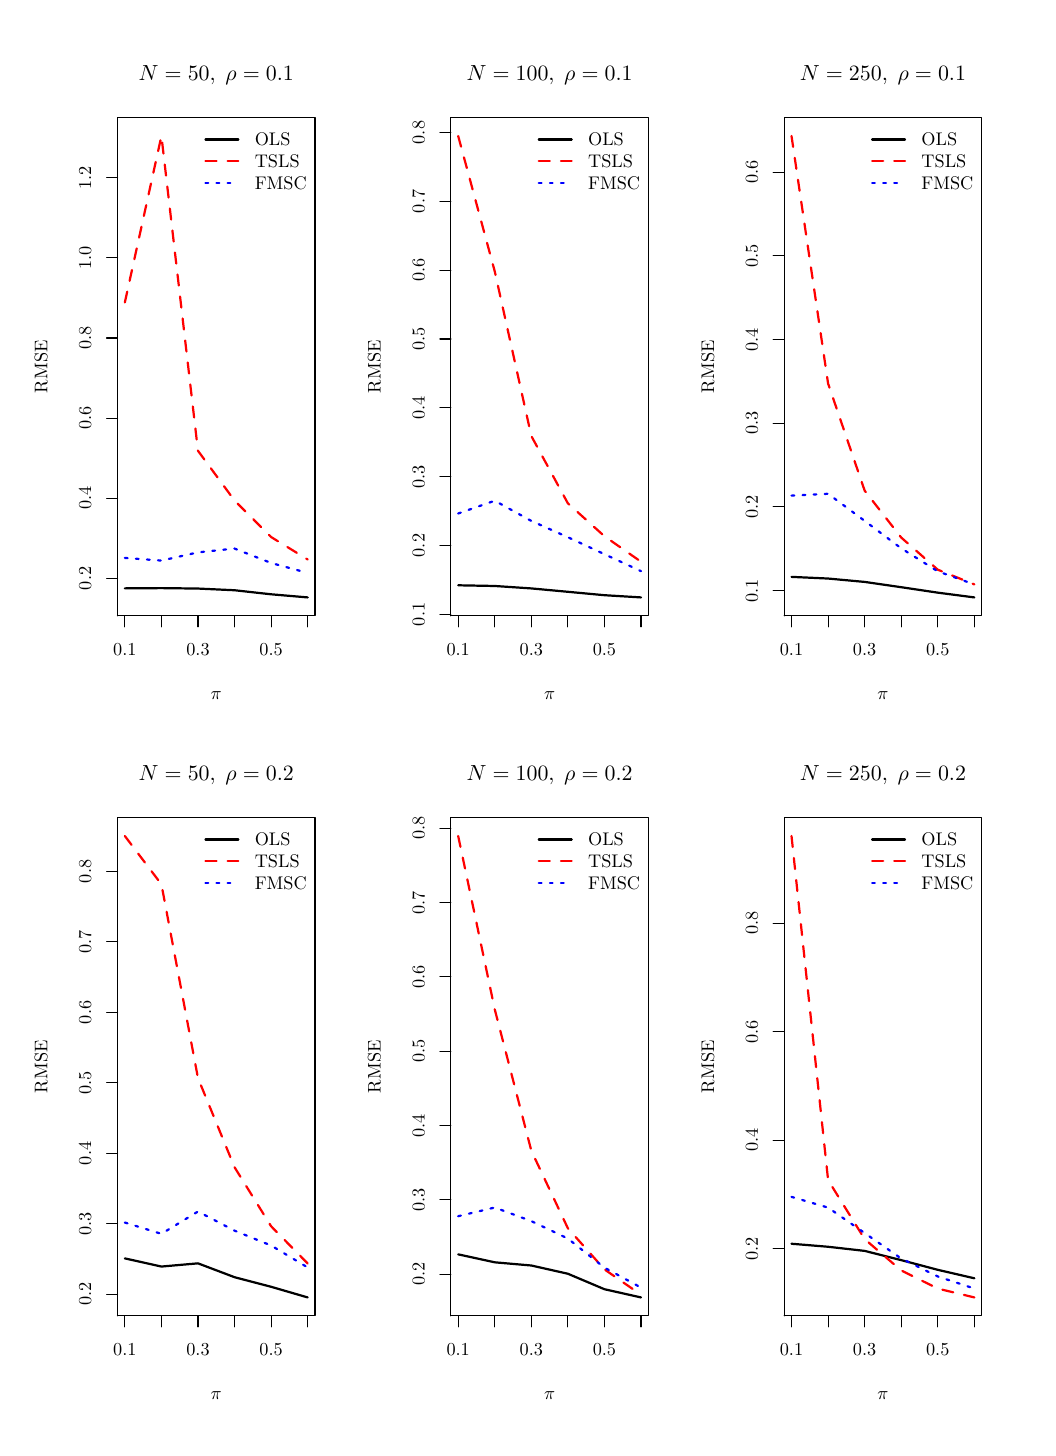
\begin{tikzpicture}[x=1pt,y=1pt]
\definecolor[named]{fillColor}{rgb}{1.00,1.00,1.00}
\path[use as bounding box,fill=fillColor,fill opacity=0.00] (0,0) rectangle (361.35,505.89);
\begin{scope}
\path[clip] ( 32.47,293.34) rectangle (103.82,473.42);
\definecolor[named]{drawColor}{rgb}{0.00,0.00,0.00}

\path[draw=drawColor,line width= 0.8pt,line join=round,line cap=round] ( 35.11,303.28) --
	( 48.33,303.37) --
	( 61.54,303.21) --
	( 74.75,302.60) --
	( 87.96,301.14) --
	(101.18,300.01);
\end{scope}
\begin{scope}
\path[clip] (  0.00,  0.00) rectangle (361.35,505.89);
\definecolor[named]{drawColor}{rgb}{0.00,0.00,0.00}

\path[draw=drawColor,line width= 0.4pt,line join=round,line cap=round] ( 35.11,293.34) -- (101.18,293.34);

\path[draw=drawColor,line width= 0.4pt,line join=round,line cap=round] ( 35.11,293.34) -- ( 35.11,289.38);

\path[draw=drawColor,line width= 0.4pt,line join=round,line cap=round] ( 48.33,293.34) -- ( 48.33,289.38);

\path[draw=drawColor,line width= 0.4pt,line join=round,line cap=round] ( 61.54,293.34) -- ( 61.54,289.38);

\path[draw=drawColor,line width= 0.4pt,line join=round,line cap=round] ( 74.75,293.34) -- ( 74.75,289.38);

\path[draw=drawColor,line width= 0.4pt,line join=round,line cap=round] ( 87.96,293.34) -- ( 87.96,289.38);

\path[draw=drawColor,line width= 0.4pt,line join=round,line cap=round] (101.18,293.34) -- (101.18,289.38);

\node[text=drawColor,anchor=base,inner sep=0pt, outer sep=0pt, scale=  0.66] at ( 35.11,279.08) {0.1};

\node[text=drawColor,anchor=base,inner sep=0pt, outer sep=0pt, scale=  0.66] at ( 61.54,279.08) {0.3};

\node[text=drawColor,anchor=base,inner sep=0pt, outer sep=0pt, scale=  0.66] at ( 87.96,279.08) {0.5};

\path[draw=drawColor,line width= 0.4pt,line join=round,line cap=round] ( 32.47,306.90) -- ( 32.47,451.64);

\path[draw=drawColor,line width= 0.4pt,line join=round,line cap=round] ( 32.47,306.90) -- ( 28.51,306.90);

\path[draw=drawColor,line width= 0.4pt,line join=round,line cap=round] ( 32.47,335.85) -- ( 28.51,335.85);

\path[draw=drawColor,line width= 0.4pt,line join=round,line cap=round] ( 32.47,364.80) -- ( 28.51,364.80);

\path[draw=drawColor,line width= 0.4pt,line join=round,line cap=round] ( 32.47,393.74) -- ( 28.51,393.74);

\path[draw=drawColor,line width= 0.4pt,line join=round,line cap=round] ( 32.47,422.69) -- ( 28.51,422.69);

\path[draw=drawColor,line width= 0.4pt,line join=round,line cap=round] ( 32.47,451.64) -- ( 28.51,451.64);

\node[text=drawColor,rotate= 90.00,anchor=base,inner sep=0pt, outer sep=0pt, scale=  0.66] at ( 22.97,306.90) {0.2};

\node[text=drawColor,rotate= 90.00,anchor=base,inner sep=0pt, outer sep=0pt, scale=  0.66] at ( 22.97,335.85) {0.4};

\node[text=drawColor,rotate= 90.00,anchor=base,inner sep=0pt, outer sep=0pt, scale=  0.66] at ( 22.97,364.80) {0.6};

\node[text=drawColor,rotate= 90.00,anchor=base,inner sep=0pt, outer sep=0pt, scale=  0.66] at ( 22.97,393.74) {0.8};

\node[text=drawColor,rotate= 90.00,anchor=base,inner sep=0pt, outer sep=0pt, scale=  0.66] at ( 22.97,422.69) {1.0};

\node[text=drawColor,rotate= 90.00,anchor=base,inner sep=0pt, outer sep=0pt, scale=  0.66] at ( 22.97,451.64) {1.2};

\path[draw=drawColor,line width= 0.4pt,line join=round,line cap=round] ( 32.47,293.34) --
	(103.82,293.34) --
	(103.82,473.42) --
	( 32.47,473.42) --
	( 32.47,293.34);
\end{scope}
\begin{scope}
\path[clip] (  0.00,252.94) rectangle (120.45,505.89);
\definecolor[named]{drawColor}{rgb}{0.00,0.00,0.00}

\node[text=drawColor,anchor=base,inner sep=0pt, outer sep=0pt, scale=  0.79] at ( 68.14,486.92) {\bfseries $N=50, \;\rho=0.1$};

\node[text=drawColor,anchor=base,inner sep=0pt, outer sep=0pt, scale=  0.66] at ( 68.14,263.24) {$\pi$};

\node[text=drawColor,rotate= 90.00,anchor=base,inner sep=0pt, outer sep=0pt, scale=  0.66] at (  7.13,383.38) {RMSE};
\end{scope}
\begin{scope}
\path[clip] ( 32.47,293.34) rectangle (103.82,473.42);
\definecolor[named]{drawColor}{rgb}{1.00,0.00,0.00}

\path[draw=drawColor,line width= 0.8pt,dash pattern=on 4pt off 4pt ,line join=round,line cap=round] ( 35.11,406.59) --
	( 48.33,466.75) --
	( 61.54,352.99) --
	( 74.75,335.02) --
	( 87.96,321.83) --
	(101.18,313.71);
\definecolor[named]{drawColor}{rgb}{0.00,0.00,1.00}

\path[draw=drawColor,line width= 0.8pt,dash pattern=on 1pt off 3pt ,line join=round,line cap=round] ( 35.11,314.28) --
	( 48.33,313.32) --
	( 61.54,316.29) --
	( 74.75,317.66) --
	( 87.96,312.45) --
	(101.18,308.86);
\definecolor[named]{drawColor}{rgb}{0.00,0.00,0.00}

\path[draw=drawColor,line width= 0.8pt,line join=round,line cap=round] ( 64.24,465.50) -- ( 76.12,465.50);
\definecolor[named]{drawColor}{rgb}{1.00,0.00,0.00}

\path[draw=drawColor,line width= 0.8pt,dash pattern=on 4pt off 4pt ,line join=round,line cap=round] ( 64.24,457.58) -- ( 76.12,457.58);
\definecolor[named]{drawColor}{rgb}{0.00,0.00,1.00}

\path[draw=drawColor,line width= 0.8pt,dash pattern=on 1pt off 3pt ,line join=round,line cap=round] ( 64.24,449.66) -- ( 76.12,449.66);
\definecolor[named]{drawColor}{rgb}{0.00,0.00,0.00}

\node[text=drawColor,anchor=base west,inner sep=0pt, outer sep=0pt, scale=  0.66] at ( 82.06,463.23) {OLS};

\node[text=drawColor,anchor=base west,inner sep=0pt, outer sep=0pt, scale=  0.66] at ( 82.06,455.31) {TSLS};

\node[text=drawColor,anchor=base west,inner sep=0pt, outer sep=0pt, scale=  0.66] at ( 82.06,447.39) {FMSC};
\end{scope}
\begin{scope}
\path[clip] ( 32.47, 40.39) rectangle (103.82,220.47);
\definecolor[named]{drawColor}{rgb}{0.00,0.00,0.00}

\path[draw=drawColor,line width= 0.8pt,line join=round,line cap=round] ( 35.11, 61.17) --
	( 48.33, 58.22) --
	( 61.54, 59.38) --
	( 74.75, 54.37) --
	( 87.96, 50.91) --
	(101.18, 47.06);
\end{scope}
\begin{scope}
\path[clip] (  0.00,  0.00) rectangle (361.35,505.89);
\definecolor[named]{drawColor}{rgb}{0.00,0.00,0.00}

\path[draw=drawColor,line width= 0.4pt,line join=round,line cap=round] ( 35.11, 40.39) -- (101.18, 40.39);

\path[draw=drawColor,line width= 0.4pt,line join=round,line cap=round] ( 35.11, 40.39) -- ( 35.11, 36.43);

\path[draw=drawColor,line width= 0.4pt,line join=round,line cap=round] ( 48.33, 40.39) -- ( 48.33, 36.43);

\path[draw=drawColor,line width= 0.4pt,line join=round,line cap=round] ( 61.54, 40.39) -- ( 61.54, 36.43);

\path[draw=drawColor,line width= 0.4pt,line join=round,line cap=round] ( 74.75, 40.39) -- ( 74.75, 36.43);

\path[draw=drawColor,line width= 0.4pt,line join=round,line cap=round] ( 87.96, 40.39) -- ( 87.96, 36.43);

\path[draw=drawColor,line width= 0.4pt,line join=round,line cap=round] (101.18, 40.39) -- (101.18, 36.43);

\node[text=drawColor,anchor=base,inner sep=0pt, outer sep=0pt, scale=  0.66] at ( 35.11, 26.14) {0.1};

\node[text=drawColor,anchor=base,inner sep=0pt, outer sep=0pt, scale=  0.66] at ( 61.54, 26.14) {0.3};

\node[text=drawColor,anchor=base,inner sep=0pt, outer sep=0pt, scale=  0.66] at ( 87.96, 26.14) {0.5};

\path[draw=drawColor,line width= 0.4pt,line join=round,line cap=round] ( 32.47, 48.19) -- ( 32.47,201.00);

\path[draw=drawColor,line width= 0.4pt,line join=round,line cap=round] ( 32.47, 48.19) -- ( 28.51, 48.19);

\path[draw=drawColor,line width= 0.4pt,line join=round,line cap=round] ( 32.47, 73.66) -- ( 28.51, 73.66);

\path[draw=drawColor,line width= 0.4pt,line join=round,line cap=round] ( 32.47, 99.13) -- ( 28.51, 99.13);

\path[draw=drawColor,line width= 0.4pt,line join=round,line cap=round] ( 32.47,124.60) -- ( 28.51,124.60);

\path[draw=drawColor,line width= 0.4pt,line join=round,line cap=round] ( 32.47,150.07) -- ( 28.51,150.07);

\path[draw=drawColor,line width= 0.4pt,line join=round,line cap=round] ( 32.47,175.54) -- ( 28.51,175.54);

\path[draw=drawColor,line width= 0.4pt,line join=round,line cap=round] ( 32.47,201.00) -- ( 28.51,201.00);

\node[text=drawColor,rotate= 90.00,anchor=base,inner sep=0pt, outer sep=0pt, scale=  0.66] at ( 22.97, 48.19) {0.2};

\node[text=drawColor,rotate= 90.00,anchor=base,inner sep=0pt, outer sep=0pt, scale=  0.66] at ( 22.97, 73.66) {0.3};

\node[text=drawColor,rotate= 90.00,anchor=base,inner sep=0pt, outer sep=0pt, scale=  0.66] at ( 22.97, 99.13) {0.4};

\node[text=drawColor,rotate= 90.00,anchor=base,inner sep=0pt, outer sep=0pt, scale=  0.66] at ( 22.97,124.60) {0.5};

\node[text=drawColor,rotate= 90.00,anchor=base,inner sep=0pt, outer sep=0pt, scale=  0.66] at ( 22.97,150.07) {0.6};

\node[text=drawColor,rotate= 90.00,anchor=base,inner sep=0pt, outer sep=0pt, scale=  0.66] at ( 22.97,175.54) {0.7};

\node[text=drawColor,rotate= 90.00,anchor=base,inner sep=0pt, outer sep=0pt, scale=  0.66] at ( 22.97,201.00) {0.8};

\path[draw=drawColor,line width= 0.4pt,line join=round,line cap=round] ( 32.47, 40.39) --
	(103.82, 40.39) --
	(103.82,220.47) --
	( 32.47,220.47) --
	( 32.47, 40.39);
\end{scope}
\begin{scope}
\path[clip] (  0.00,  0.00) rectangle (120.45,252.94);
\definecolor[named]{drawColor}{rgb}{0.00,0.00,0.00}

\node[text=drawColor,anchor=base,inner sep=0pt, outer sep=0pt, scale=  0.79] at ( 68.14,233.98) {\bfseries $N=50, \;\rho=0.2$};

\node[text=drawColor,anchor=base,inner sep=0pt, outer sep=0pt, scale=  0.66] at ( 68.14, 10.30) {$\pi$};

\node[text=drawColor,rotate= 90.00,anchor=base,inner sep=0pt, outer sep=0pt, scale=  0.66] at (  7.13,130.43) {RMSE};
\end{scope}
\begin{scope}
\path[clip] ( 32.47, 40.39) rectangle (103.82,220.47);
\definecolor[named]{drawColor}{rgb}{1.00,0.00,0.00}

\path[draw=drawColor,line width= 0.8pt,dash pattern=on 4pt off 4pt ,line join=round,line cap=round] ( 35.11,213.80) --
	( 48.33,196.34) --
	( 61.54,126.32) --
	( 74.75, 94.11) --
	( 87.96, 72.78) --
	(101.18, 59.33);
\definecolor[named]{drawColor}{rgb}{0.00,0.00,1.00}

\path[draw=drawColor,line width= 0.8pt,dash pattern=on 1pt off 3pt ,line join=round,line cap=round] ( 35.11, 74.12) --
	( 48.33, 70.04) --
	( 61.54, 78.11) --
	( 74.75, 71.19) --
	( 87.96, 65.83) --
	(101.18, 57.89);
\definecolor[named]{drawColor}{rgb}{0.00,0.00,0.00}

\path[draw=drawColor,line width= 0.8pt,line join=round,line cap=round] ( 64.24,212.55) -- ( 76.12,212.55);
\definecolor[named]{drawColor}{rgb}{1.00,0.00,0.00}

\path[draw=drawColor,line width= 0.8pt,dash pattern=on 4pt off 4pt ,line join=round,line cap=round] ( 64.24,204.63) -- ( 76.12,204.63);
\definecolor[named]{drawColor}{rgb}{0.00,0.00,1.00}

\path[draw=drawColor,line width= 0.8pt,dash pattern=on 1pt off 3pt ,line join=round,line cap=round] ( 64.24,196.71) -- ( 76.12,196.71);
\definecolor[named]{drawColor}{rgb}{0.00,0.00,0.00}

\node[text=drawColor,anchor=base west,inner sep=0pt, outer sep=0pt, scale=  0.66] at ( 82.06,210.28) {OLS};

\node[text=drawColor,anchor=base west,inner sep=0pt, outer sep=0pt, scale=  0.66] at ( 82.06,202.36) {TSLS};

\node[text=drawColor,anchor=base west,inner sep=0pt, outer sep=0pt, scale=  0.66] at ( 82.06,194.44) {FMSC};
\end{scope}
\begin{scope}
\path[clip] (152.92,293.34) rectangle (224.27,473.42);
\definecolor[named]{drawColor}{rgb}{0.00,0.00,0.00}

\path[draw=drawColor,line width= 0.8pt,line join=round,line cap=round] (155.56,304.39) --
	(168.78,304.14) --
	(181.99,303.26) --
	(195.20,302.04) --
	(208.41,300.81) --
	(221.63,300.01);
\end{scope}
\begin{scope}
\path[clip] (  0.00,  0.00) rectangle (361.35,505.89);
\definecolor[named]{drawColor}{rgb}{0.00,0.00,0.00}

\path[draw=drawColor,line width= 0.4pt,line join=round,line cap=round] (155.56,293.34) -- (221.63,293.34);

\path[draw=drawColor,line width= 0.4pt,line join=round,line cap=round] (155.56,293.34) -- (155.56,289.38);

\path[draw=drawColor,line width= 0.4pt,line join=round,line cap=round] (168.78,293.34) -- (168.78,289.38);

\path[draw=drawColor,line width= 0.4pt,line join=round,line cap=round] (181.99,293.34) -- (181.99,289.38);

\path[draw=drawColor,line width= 0.4pt,line join=round,line cap=round] (195.20,293.34) -- (195.20,289.38);

\path[draw=drawColor,line width= 0.4pt,line join=round,line cap=round] (208.41,293.34) -- (208.41,289.38);

\path[draw=drawColor,line width= 0.4pt,line join=round,line cap=round] (221.63,293.34) -- (221.63,289.38);

\node[text=drawColor,anchor=base,inner sep=0pt, outer sep=0pt, scale=  0.66] at (155.56,279.08) {0.1};

\node[text=drawColor,anchor=base,inner sep=0pt, outer sep=0pt, scale=  0.66] at (181.99,279.08) {0.3};

\node[text=drawColor,anchor=base,inner sep=0pt, outer sep=0pt, scale=  0.66] at (208.41,279.08) {0.5};

\path[draw=drawColor,line width= 0.4pt,line join=round,line cap=round] (152.92,293.90) -- (152.92,468.00);

\path[draw=drawColor,line width= 0.4pt,line join=round,line cap=round] (152.92,293.90) -- (148.96,293.90);

\path[draw=drawColor,line width= 0.4pt,line join=round,line cap=round] (152.92,318.77) -- (148.96,318.77);

\path[draw=drawColor,line width= 0.4pt,line join=round,line cap=round] (152.92,343.64) -- (148.96,343.64);

\path[draw=drawColor,line width= 0.4pt,line join=round,line cap=round] (152.92,368.52) -- (148.96,368.52);

\path[draw=drawColor,line width= 0.4pt,line join=round,line cap=round] (152.92,393.39) -- (148.96,393.39);

\path[draw=drawColor,line width= 0.4pt,line join=round,line cap=round] (152.92,418.26) -- (148.96,418.26);

\path[draw=drawColor,line width= 0.4pt,line join=round,line cap=round] (152.92,443.13) -- (148.96,443.13);

\path[draw=drawColor,line width= 0.4pt,line join=round,line cap=round] (152.92,468.00) -- (148.96,468.00);

\node[text=drawColor,rotate= 90.00,anchor=base,inner sep=0pt, outer sep=0pt, scale=  0.66] at (143.42,293.90) {0.1};

\node[text=drawColor,rotate= 90.00,anchor=base,inner sep=0pt, outer sep=0pt, scale=  0.66] at (143.42,318.77) {0.2};

\node[text=drawColor,rotate= 90.00,anchor=base,inner sep=0pt, outer sep=0pt, scale=  0.66] at (143.42,343.64) {0.3};

\node[text=drawColor,rotate= 90.00,anchor=base,inner sep=0pt, outer sep=0pt, scale=  0.66] at (143.42,368.52) {0.4};

\node[text=drawColor,rotate= 90.00,anchor=base,inner sep=0pt, outer sep=0pt, scale=  0.66] at (143.42,393.39) {0.5};

\node[text=drawColor,rotate= 90.00,anchor=base,inner sep=0pt, outer sep=0pt, scale=  0.66] at (143.42,418.26) {0.6};

\node[text=drawColor,rotate= 90.00,anchor=base,inner sep=0pt, outer sep=0pt, scale=  0.66] at (143.42,443.13) {0.7};

\node[text=drawColor,rotate= 90.00,anchor=base,inner sep=0pt, outer sep=0pt, scale=  0.66] at (143.42,468.00) {0.8};

\path[draw=drawColor,line width= 0.4pt,line join=round,line cap=round] (152.92,293.34) --
	(224.27,293.34) --
	(224.27,473.42) --
	(152.92,473.42) --
	(152.92,293.34);
\end{scope}
\begin{scope}
\path[clip] (120.45,252.94) rectangle (240.90,505.89);
\definecolor[named]{drawColor}{rgb}{0.00,0.00,0.00}

\node[text=drawColor,anchor=base,inner sep=0pt, outer sep=0pt, scale=  0.79] at (188.59,486.92) {\bfseries $N=100, \;\rho=0.1$};

\node[text=drawColor,anchor=base,inner sep=0pt, outer sep=0pt, scale=  0.66] at (188.59,263.24) {$\pi$};

\node[text=drawColor,rotate= 90.00,anchor=base,inner sep=0pt, outer sep=0pt, scale=  0.66] at (127.58,383.38) {RMSE};
\end{scope}
\begin{scope}
\path[clip] (152.92,293.34) rectangle (224.27,473.42);
\definecolor[named]{drawColor}{rgb}{1.00,0.00,0.00}

\path[draw=drawColor,line width= 0.8pt,dash pattern=on 4pt off 4pt ,line join=round,line cap=round] (155.56,466.75) --
	(168.78,417.80) --
	(181.99,358.33) --
	(195.20,334.00) --
	(208.41,322.12) --
	(221.63,312.91);
\definecolor[named]{drawColor}{rgb}{0.00,0.00,1.00}

\path[draw=drawColor,line width= 0.8pt,dash pattern=on 1pt off 3pt ,line join=round,line cap=round] (155.56,330.34) --
	(168.78,334.95) --
	(181.99,327.65) --
	(195.20,321.76) --
	(208.41,315.63) --
	(221.63,309.51);
\definecolor[named]{drawColor}{rgb}{0.00,0.00,0.00}

\path[draw=drawColor,line width= 0.8pt,line join=round,line cap=round] (184.69,465.50) -- (196.57,465.50);
\definecolor[named]{drawColor}{rgb}{1.00,0.00,0.00}

\path[draw=drawColor,line width= 0.8pt,dash pattern=on 4pt off 4pt ,line join=round,line cap=round] (184.69,457.58) -- (196.57,457.58);
\definecolor[named]{drawColor}{rgb}{0.00,0.00,1.00}

\path[draw=drawColor,line width= 0.8pt,dash pattern=on 1pt off 3pt ,line join=round,line cap=round] (184.69,449.66) -- (196.57,449.66);
\definecolor[named]{drawColor}{rgb}{0.00,0.00,0.00}

\node[text=drawColor,anchor=base west,inner sep=0pt, outer sep=0pt, scale=  0.66] at (202.51,463.23) {OLS};

\node[text=drawColor,anchor=base west,inner sep=0pt, outer sep=0pt, scale=  0.66] at (202.51,455.31) {TSLS};

\node[text=drawColor,anchor=base west,inner sep=0pt, outer sep=0pt, scale=  0.66] at (202.51,447.39) {FMSC};
\end{scope}
\begin{scope}
\path[clip] (152.92, 40.39) rectangle (224.27,220.47);
\definecolor[named]{drawColor}{rgb}{0.00,0.00,0.00}

\path[draw=drawColor,line width= 0.8pt,line join=round,line cap=round] (155.56, 62.63) --
	(168.78, 59.75) --
	(181.99, 58.60) --
	(195.20, 55.62) --
	(208.41, 50.03) --
	(221.63, 47.06);
\end{scope}
\begin{scope}
\path[clip] (  0.00,  0.00) rectangle (361.35,505.89);
\definecolor[named]{drawColor}{rgb}{0.00,0.00,0.00}

\path[draw=drawColor,line width= 0.4pt,line join=round,line cap=round] (155.56, 40.39) -- (221.63, 40.39);

\path[draw=drawColor,line width= 0.4pt,line join=round,line cap=round] (155.56, 40.39) -- (155.56, 36.43);

\path[draw=drawColor,line width= 0.4pt,line join=round,line cap=round] (168.78, 40.39) -- (168.78, 36.43);

\path[draw=drawColor,line width= 0.4pt,line join=round,line cap=round] (181.99, 40.39) -- (181.99, 36.43);

\path[draw=drawColor,line width= 0.4pt,line join=round,line cap=round] (195.20, 40.39) -- (195.20, 36.43);

\path[draw=drawColor,line width= 0.4pt,line join=round,line cap=round] (208.41, 40.39) -- (208.41, 36.43);

\path[draw=drawColor,line width= 0.4pt,line join=round,line cap=round] (221.63, 40.39) -- (221.63, 36.43);

\node[text=drawColor,anchor=base,inner sep=0pt, outer sep=0pt, scale=  0.66] at (155.56, 26.14) {0.1};

\node[text=drawColor,anchor=base,inner sep=0pt, outer sep=0pt, scale=  0.66] at (181.99, 26.14) {0.3};

\node[text=drawColor,anchor=base,inner sep=0pt, outer sep=0pt, scale=  0.66] at (208.41, 26.14) {0.5};

\path[draw=drawColor,line width= 0.4pt,line join=round,line cap=round] (152.92, 55.46) -- (152.92,216.60);

\path[draw=drawColor,line width= 0.4pt,line join=round,line cap=round] (152.92, 55.46) -- (148.96, 55.46);

\path[draw=drawColor,line width= 0.4pt,line join=round,line cap=round] (152.92, 82.31) -- (148.96, 82.31);

\path[draw=drawColor,line width= 0.4pt,line join=round,line cap=round] (152.92,109.17) -- (148.96,109.17);

\path[draw=drawColor,line width= 0.4pt,line join=round,line cap=round] (152.92,136.03) -- (148.96,136.03);

\path[draw=drawColor,line width= 0.4pt,line join=round,line cap=round] (152.92,162.89) -- (148.96,162.89);

\path[draw=drawColor,line width= 0.4pt,line join=round,line cap=round] (152.92,189.75) -- (148.96,189.75);

\path[draw=drawColor,line width= 0.4pt,line join=round,line cap=round] (152.92,216.60) -- (148.96,216.60);

\node[text=drawColor,rotate= 90.00,anchor=base,inner sep=0pt, outer sep=0pt, scale=  0.66] at (143.42, 55.46) {0.2};

\node[text=drawColor,rotate= 90.00,anchor=base,inner sep=0pt, outer sep=0pt, scale=  0.66] at (143.42, 82.31) {0.3};

\node[text=drawColor,rotate= 90.00,anchor=base,inner sep=0pt, outer sep=0pt, scale=  0.66] at (143.42,109.17) {0.4};

\node[text=drawColor,rotate= 90.00,anchor=base,inner sep=0pt, outer sep=0pt, scale=  0.66] at (143.42,136.03) {0.5};

\node[text=drawColor,rotate= 90.00,anchor=base,inner sep=0pt, outer sep=0pt, scale=  0.66] at (143.42,162.89) {0.6};

\node[text=drawColor,rotate= 90.00,anchor=base,inner sep=0pt, outer sep=0pt, scale=  0.66] at (143.42,189.75) {0.7};

\node[text=drawColor,rotate= 90.00,anchor=base,inner sep=0pt, outer sep=0pt, scale=  0.66] at (143.42,216.60) {0.8};

\path[draw=drawColor,line width= 0.4pt,line join=round,line cap=round] (152.92, 40.39) --
	(224.27, 40.39) --
	(224.27,220.47) --
	(152.92,220.47) --
	(152.92, 40.39);
\end{scope}
\begin{scope}
\path[clip] (120.45,  0.00) rectangle (240.90,252.94);
\definecolor[named]{drawColor}{rgb}{0.00,0.00,0.00}

\node[text=drawColor,anchor=base,inner sep=0pt, outer sep=0pt, scale=  0.79] at (188.59,233.98) {\bfseries $N=100, \;\rho=0.2$};

\node[text=drawColor,anchor=base,inner sep=0pt, outer sep=0pt, scale=  0.66] at (188.59, 10.30) {$\pi$};

\node[text=drawColor,rotate= 90.00,anchor=base,inner sep=0pt, outer sep=0pt, scale=  0.66] at (127.58,130.43) {RMSE};
\end{scope}
\begin{scope}
\path[clip] (152.92, 40.39) rectangle (224.27,220.47);
\definecolor[named]{drawColor}{rgb}{1.00,0.00,0.00}

\path[draw=drawColor,line width= 0.8pt,dash pattern=on 4pt off 4pt ,line join=round,line cap=round] (155.56,213.80) --
	(168.78,151.14) --
	(181.99,100.08) --
	(195.20, 72.05) --
	(208.41, 57.20) --
	(221.63, 48.03);
\definecolor[named]{drawColor}{rgb}{0.00,0.00,1.00}

\path[draw=drawColor,line width= 0.8pt,dash pattern=on 1pt off 3pt ,line join=round,line cap=round] (155.56, 76.41) --
	(168.78, 79.55) --
	(181.99, 74.64) --
	(195.20, 68.33) --
	(208.41, 57.83) --
	(221.63, 50.62);
\definecolor[named]{drawColor}{rgb}{0.00,0.00,0.00}

\path[draw=drawColor,line width= 0.8pt,line join=round,line cap=round] (184.69,212.55) -- (196.57,212.55);
\definecolor[named]{drawColor}{rgb}{1.00,0.00,0.00}

\path[draw=drawColor,line width= 0.8pt,dash pattern=on 4pt off 4pt ,line join=round,line cap=round] (184.69,204.63) -- (196.57,204.63);
\definecolor[named]{drawColor}{rgb}{0.00,0.00,1.00}

\path[draw=drawColor,line width= 0.8pt,dash pattern=on 1pt off 3pt ,line join=round,line cap=round] (184.69,196.71) -- (196.57,196.71);
\definecolor[named]{drawColor}{rgb}{0.00,0.00,0.00}

\node[text=drawColor,anchor=base west,inner sep=0pt, outer sep=0pt, scale=  0.66] at (202.51,210.28) {OLS};

\node[text=drawColor,anchor=base west,inner sep=0pt, outer sep=0pt, scale=  0.66] at (202.51,202.36) {TSLS};

\node[text=drawColor,anchor=base west,inner sep=0pt, outer sep=0pt, scale=  0.66] at (202.51,194.44) {FMSC};
\end{scope}
\begin{scope}
\path[clip] (273.37,293.34) rectangle (344.72,473.42);
\definecolor[named]{drawColor}{rgb}{0.00,0.00,0.00}

\path[draw=drawColor,line width= 0.8pt,line join=round,line cap=round] (276.01,307.43) --
	(289.23,306.83) --
	(302.44,305.61) --
	(315.65,303.70) --
	(328.86,301.73) --
	(342.08,300.01);
\end{scope}
\begin{scope}
\path[clip] (  0.00,  0.00) rectangle (361.35,505.89);
\definecolor[named]{drawColor}{rgb}{0.00,0.00,0.00}

\path[draw=drawColor,line width= 0.4pt,line join=round,line cap=round] (276.01,293.34) -- (342.08,293.34);

\path[draw=drawColor,line width= 0.4pt,line join=round,line cap=round] (276.01,293.34) -- (276.01,289.38);

\path[draw=drawColor,line width= 0.4pt,line join=round,line cap=round] (289.23,293.34) -- (289.23,289.38);

\path[draw=drawColor,line width= 0.4pt,line join=round,line cap=round] (302.44,293.34) -- (302.44,289.38);

\path[draw=drawColor,line width= 0.4pt,line join=round,line cap=round] (315.65,293.34) -- (315.65,289.38);

\path[draw=drawColor,line width= 0.4pt,line join=round,line cap=round] (328.86,293.34) -- (328.86,289.38);

\path[draw=drawColor,line width= 0.4pt,line join=round,line cap=round] (342.08,293.34) -- (342.08,289.38);

\node[text=drawColor,anchor=base,inner sep=0pt, outer sep=0pt, scale=  0.66] at (276.01,279.08) {0.1};

\node[text=drawColor,anchor=base,inner sep=0pt, outer sep=0pt, scale=  0.66] at (302.44,279.08) {0.3};

\node[text=drawColor,anchor=base,inner sep=0pt, outer sep=0pt, scale=  0.66] at (328.86,279.08) {0.5};

\path[draw=drawColor,line width= 0.4pt,line join=round,line cap=round] (273.37,302.46) -- (273.37,453.67);

\path[draw=drawColor,line width= 0.4pt,line join=round,line cap=round] (273.37,302.46) -- (269.41,302.46);

\path[draw=drawColor,line width= 0.4pt,line join=round,line cap=round] (273.37,332.70) -- (269.41,332.70);

\path[draw=drawColor,line width= 0.4pt,line join=round,line cap=round] (273.37,362.94) -- (269.41,362.94);

\path[draw=drawColor,line width= 0.4pt,line join=round,line cap=round] (273.37,393.19) -- (269.41,393.19);

\path[draw=drawColor,line width= 0.4pt,line join=round,line cap=round] (273.37,423.43) -- (269.41,423.43);

\path[draw=drawColor,line width= 0.4pt,line join=round,line cap=round] (273.37,453.67) -- (269.41,453.67);

\node[text=drawColor,rotate= 90.00,anchor=base,inner sep=0pt, outer sep=0pt, scale=  0.66] at (263.87,302.46) {0.1};

\node[text=drawColor,rotate= 90.00,anchor=base,inner sep=0pt, outer sep=0pt, scale=  0.66] at (263.87,332.70) {0.2};

\node[text=drawColor,rotate= 90.00,anchor=base,inner sep=0pt, outer sep=0pt, scale=  0.66] at (263.87,362.94) {0.3};

\node[text=drawColor,rotate= 90.00,anchor=base,inner sep=0pt, outer sep=0pt, scale=  0.66] at (263.87,393.19) {0.4};

\node[text=drawColor,rotate= 90.00,anchor=base,inner sep=0pt, outer sep=0pt, scale=  0.66] at (263.87,423.43) {0.5};

\node[text=drawColor,rotate= 90.00,anchor=base,inner sep=0pt, outer sep=0pt, scale=  0.66] at (263.87,453.67) {0.6};

\path[draw=drawColor,line width= 0.4pt,line join=round,line cap=round] (273.37,293.34) --
	(344.72,293.34) --
	(344.72,473.42) --
	(273.37,473.42) --
	(273.37,293.34);
\end{scope}
\begin{scope}
\path[clip] (240.90,252.94) rectangle (361.35,505.89);
\definecolor[named]{drawColor}{rgb}{0.00,0.00,0.00}

\node[text=drawColor,anchor=base,inner sep=0pt, outer sep=0pt, scale=  0.79] at (309.04,486.92) {\bfseries $N=250, \;\rho=0.1$};

\node[text=drawColor,anchor=base,inner sep=0pt, outer sep=0pt, scale=  0.66] at (309.04,263.24) {$\pi$};

\node[text=drawColor,rotate= 90.00,anchor=base,inner sep=0pt, outer sep=0pt, scale=  0.66] at (248.03,383.38) {RMSE};
\end{scope}
\begin{scope}
\path[clip] (273.37,293.34) rectangle (344.72,473.42);
\definecolor[named]{drawColor}{rgb}{1.00,0.00,0.00}

\path[draw=drawColor,line width= 0.8pt,dash pattern=on 4pt off 4pt ,line join=round,line cap=round] (276.01,466.75) --
	(289.23,377.28) --
	(302.44,338.59) --
	(315.65,321.64) --
	(328.86,310.03) --
	(342.08,304.71);
\definecolor[named]{drawColor}{rgb}{0.00,0.00,1.00}

\path[draw=drawColor,line width= 0.8pt,dash pattern=on 1pt off 3pt ,line join=round,line cap=round] (276.01,336.79) --
	(289.23,337.46) --
	(302.44,327.67) --
	(315.65,317.75) --
	(328.86,309.44) --
	(342.08,304.70);
\definecolor[named]{drawColor}{rgb}{0.00,0.00,0.00}

\path[draw=drawColor,line width= 0.8pt,line join=round,line cap=round] (305.14,465.50) -- (317.02,465.50);
\definecolor[named]{drawColor}{rgb}{1.00,0.00,0.00}

\path[draw=drawColor,line width= 0.8pt,dash pattern=on 4pt off 4pt ,line join=round,line cap=round] (305.14,457.58) -- (317.02,457.58);
\definecolor[named]{drawColor}{rgb}{0.00,0.00,1.00}

\path[draw=drawColor,line width= 0.8pt,dash pattern=on 1pt off 3pt ,line join=round,line cap=round] (305.14,449.66) -- (317.02,449.66);
\definecolor[named]{drawColor}{rgb}{0.00,0.00,0.00}

\node[text=drawColor,anchor=base west,inner sep=0pt, outer sep=0pt, scale=  0.66] at (322.96,463.23) {OLS};

\node[text=drawColor,anchor=base west,inner sep=0pt, outer sep=0pt, scale=  0.66] at (322.96,455.31) {TSLS};

\node[text=drawColor,anchor=base west,inner sep=0pt, outer sep=0pt, scale=  0.66] at (322.96,447.39) {FMSC};
\end{scope}
\begin{scope}
\path[clip] (273.37, 40.39) rectangle (344.72,220.47);
\definecolor[named]{drawColor}{rgb}{0.00,0.00,0.00}

\path[draw=drawColor,line width= 0.8pt,line join=round,line cap=round] (276.01, 66.46) --
	(289.23, 65.37) --
	(302.44, 63.88) --
	(315.65, 60.54) --
	(328.86, 57.04) --
	(342.08, 53.98);
\end{scope}
\begin{scope}
\path[clip] (  0.00,  0.00) rectangle (361.35,505.89);
\definecolor[named]{drawColor}{rgb}{0.00,0.00,0.00}

\path[draw=drawColor,line width= 0.4pt,line join=round,line cap=round] (276.01, 40.39) -- (342.08, 40.39);

\path[draw=drawColor,line width= 0.4pt,line join=round,line cap=round] (276.01, 40.39) -- (276.01, 36.43);

\path[draw=drawColor,line width= 0.4pt,line join=round,line cap=round] (289.23, 40.39) -- (289.23, 36.43);

\path[draw=drawColor,line width= 0.4pt,line join=round,line cap=round] (302.44, 40.39) -- (302.44, 36.43);

\path[draw=drawColor,line width= 0.4pt,line join=round,line cap=round] (315.65, 40.39) -- (315.65, 36.43);

\path[draw=drawColor,line width= 0.4pt,line join=round,line cap=round] (328.86, 40.39) -- (328.86, 36.43);

\path[draw=drawColor,line width= 0.4pt,line join=round,line cap=round] (342.08, 40.39) -- (342.08, 36.43);

\node[text=drawColor,anchor=base,inner sep=0pt, outer sep=0pt, scale=  0.66] at (276.01, 26.14) {0.1};

\node[text=drawColor,anchor=base,inner sep=0pt, outer sep=0pt, scale=  0.66] at (302.44, 26.14) {0.3};

\node[text=drawColor,anchor=base,inner sep=0pt, outer sep=0pt, scale=  0.66] at (328.86, 26.14) {0.5};

\path[draw=drawColor,line width= 0.4pt,line join=round,line cap=round] (273.37, 64.61) -- (273.37,182.30);

\path[draw=drawColor,line width= 0.4pt,line join=round,line cap=round] (273.37, 64.61) -- (269.41, 64.61);

\path[draw=drawColor,line width= 0.4pt,line join=round,line cap=round] (273.37,103.84) -- (269.41,103.84);

\path[draw=drawColor,line width= 0.4pt,line join=round,line cap=round] (273.37,143.07) -- (269.41,143.07);

\path[draw=drawColor,line width= 0.4pt,line join=round,line cap=round] (273.37,182.30) -- (269.41,182.30);

\node[text=drawColor,rotate= 90.00,anchor=base,inner sep=0pt, outer sep=0pt, scale=  0.66] at (263.87, 64.61) {0.2};

\node[text=drawColor,rotate= 90.00,anchor=base,inner sep=0pt, outer sep=0pt, scale=  0.66] at (263.87,103.84) {0.4};

\node[text=drawColor,rotate= 90.00,anchor=base,inner sep=0pt, outer sep=0pt, scale=  0.66] at (263.87,143.07) {0.6};

\node[text=drawColor,rotate= 90.00,anchor=base,inner sep=0pt, outer sep=0pt, scale=  0.66] at (263.87,182.30) {0.8};

\path[draw=drawColor,line width= 0.4pt,line join=round,line cap=round] (273.37, 40.39) --
	(344.72, 40.39) --
	(344.72,220.47) --
	(273.37,220.47) --
	(273.37, 40.39);
\end{scope}
\begin{scope}
\path[clip] (240.90,  0.00) rectangle (361.35,252.94);
\definecolor[named]{drawColor}{rgb}{0.00,0.00,0.00}

\node[text=drawColor,anchor=base,inner sep=0pt, outer sep=0pt, scale=  0.79] at (309.04,233.98) {\bfseries $N=250, \;\rho=0.2$};

\node[text=drawColor,anchor=base,inner sep=0pt, outer sep=0pt, scale=  0.66] at (309.04, 10.30) {$\pi$};

\node[text=drawColor,rotate= 90.00,anchor=base,inner sep=0pt, outer sep=0pt, scale=  0.66] at (248.03,130.43) {RMSE};
\end{scope}
\begin{scope}
\path[clip] (273.37, 40.39) rectangle (344.72,220.47);
\definecolor[named]{drawColor}{rgb}{1.00,0.00,0.00}

\path[draw=drawColor,line width= 0.8pt,dash pattern=on 4pt off 4pt ,line join=round,line cap=round] (276.01,213.80) --
	(289.23, 89.46) --
	(302.44, 68.13) --
	(315.65, 56.82) --
	(328.86, 50.26) --
	(342.08, 47.06);
\definecolor[named]{drawColor}{rgb}{0.00,0.00,1.00}

\path[draw=drawColor,line width= 0.8pt,dash pattern=on 1pt off 3pt ,line join=round,line cap=round] (276.01, 83.40) --
	(289.23, 79.52) --
	(302.44, 70.33) --
	(315.65, 61.13) --
	(328.86, 54.64) --
	(342.08, 50.28);
\definecolor[named]{drawColor}{rgb}{0.00,0.00,0.00}

\path[draw=drawColor,line width= 0.8pt,line join=round,line cap=round] (305.14,212.55) -- (317.02,212.55);
\definecolor[named]{drawColor}{rgb}{1.00,0.00,0.00}

\path[draw=drawColor,line width= 0.8pt,dash pattern=on 4pt off 4pt ,line join=round,line cap=round] (305.14,204.63) -- (317.02,204.63);
\definecolor[named]{drawColor}{rgb}{0.00,0.00,1.00}

\path[draw=drawColor,line width= 0.8pt,dash pattern=on 1pt off 3pt ,line join=round,line cap=round] (305.14,196.71) -- (317.02,196.71);
\definecolor[named]{drawColor}{rgb}{0.00,0.00,0.00}

\node[text=drawColor,anchor=base west,inner sep=0pt, outer sep=0pt, scale=  0.66] at (322.96,210.28) {OLS};

\node[text=drawColor,anchor=base west,inner sep=0pt, outer sep=0pt, scale=  0.66] at (322.96,202.36) {TSLS};

\node[text=drawColor,anchor=base west,inner sep=0pt, outer sep=0pt, scale=  0.66] at (322.96,194.44) {FMSC};
\end{scope}
\end{tikzpicture}
